\section{Affine reconstruction}

\begin{theorem}
    A projective transformation $H$ that maps the line at the infinity $l_{\infty}$ onto itself implies that $H$ is affine. 
\end{theorem}
\begin{proof}
    A point at the infinity $x_{\infty}={\begin{bmatrix} x & y & 0 \end{bmatrix}^T}$ is mapped to another point $x^{'}=Hx_{\infty}$ that remains at infinity only if the third coordinate of $x'$ is zero.
    For all $(x,y)$, this condition is expressed as:
    \[\begin{bmatrix} v_1 & v_2 & 1 \end{bmatrix} \begin{bmatrix} x \\ y \\ 0 \end{bmatrix}=0 \rightarrow \begin{bmatrix} v_1 & v_2 & 1 \end{bmatrix} = \begin{bmatrix} 0 & 0 & 1 \end{bmatrix}\]
    In other words, $H$ is affine.
\end{proof}
The image provided results from a general projective mapping of the original scene. 
Consequently, the vanishing line $l^{'}_{\infty}$ in the image differs from the original $l_{\infty}$. 
This observation leads to the possibility of using $l^{'}_{\infty}$ as additional information.
By applying a new projective transformation $H_{AR}$ to the image that restores $l^{'}_{\infty}$ to $l_{\infty}$, a modified image is obtained.
Notably, the image of the line at infinity $l_{\infty}$ in this new model remains as $l_{\infty}$. 

Based on the theorem, the resulting model (i.e., the new image) is an affine mapping of the original scene. 
Therefore, the achieved model is an affine reconstruction of the scene.
\begin{figure}[H]
    \centering
    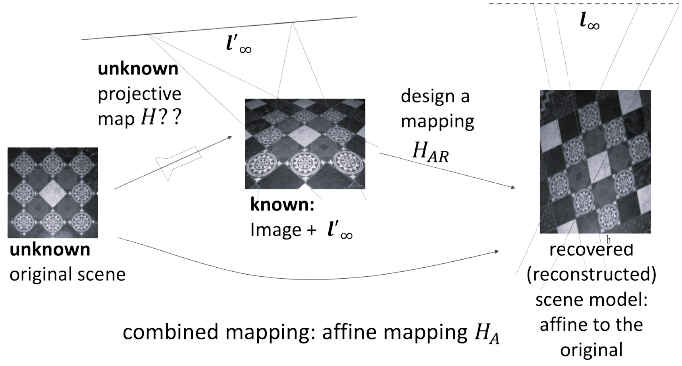
\includegraphics[width=0.75\linewidth]{images/HAR.png}
\end{figure}
The challenges associated with this approach include:
\begin{itemize}
    \item Determine a projective transformation $H_{AR}$ that restores $l^{'}_{\infty}$ to $l_{\infty}$.
    \item Identify the vanishing line.
\end{itemize}

\subsection*{Determine a projective transformation}
To find a projective mapping $H_{AR}$ that restores $l^{'}_{\infty}$ to $l_{\infty}$ the mapping should satisfy the condition of mapping any point $x^{'} \in l^{'}_{\infty}$ onto a set of point at infinity: 
\[H_{AR}x^{'} = \begin{bmatrix} * \\ * \\ 0 \end{bmatrix}\]
The mapping can be effectively represented as:
\[H_{AR}=
\begin{bmatrix}
    * & * & * \\
    * & * & * \\
    \: & l^{'T}_{\infty} & \:
\end{bmatrix}\]
In this matrix representation, we achieve the desired mapping: 
\[H_{AR}x^{'}=
\begin{bmatrix}
    * & * & * \\
    * & * & * \\
    \: & l^{'T}_{\infty} & \:
\end{bmatrix}
x^{'}
=
\begin{bmatrix}
    * \\
    * \\
    l^{'T}_{\infty}x^{'}
\end{bmatrix}
\]

\subsection*{Identify the vanishing line}
To determine the vanishing line, additional information can be employed, such as the image of parallel lines.
\begin{figure}[H]
    \centering
    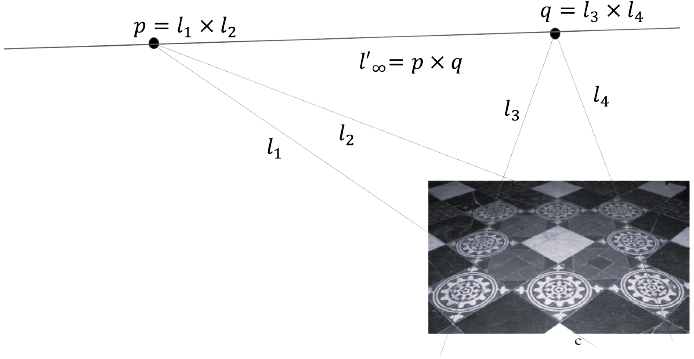
\includegraphics[width=0.5\linewidth]{images/van.png}
\end{figure}